\chapter{Methods}
In this thesis, I analyze a dataset comprising the properties of a sample of galaxies from the Seventh Data Release (DR7) of the Sloan Digital Sky Survey. Covering 11,663 square degrees of imaging data, DR7 offers extensive five-band photometry for 357 million celestial objects \cite{2009ApJS..182..543A,mpa-sdss-dr7}. 

As shown in  \autoref{3}, the Legacy imaging footprint is depicted as the extensive contiguous gray area on the left side of the upper panel, complemented by three separated gray stripes visible on the right side.

With completed spectroscopy over 9380 square degrees, including 1.6 million spectra of galaxies, quasars, and stars, the SDSS DR7 dataset serves as the primary catalog for this study. A depiction of the spectroscopic coverage is shown in the lower panel of \autoref{3} 
 
I will focus on following physical properties : \textbf{Redshift} and \textbf{Integrated flux with their relative uncertainties} of the common optical lines (i.e. $H\alpha$, $H\beta$...).

In the context of SDSS DR7, these properties are calculated using an automated procedure of gaussian fitting, applied in two subsequent moments. In the first phase the object is classified and redshift is calculated by fitting at the same moment only the emission lines, while in the second part of the procedure this computation is extended to all lines available. It is important to note that \textbf{each} line is \textbf{individually fitted as a single Gaussian} on the continuum-subtracted spectrum, with modalities presented by O'Donnell \cite{1994ApJ...422..158O}. Information on the Radio classification of the galaxies in this sample is obtained from FIRST and NVSS images from Best et Al. \cite{2005MNRAS.362....9B}.

\begin{comment}
the line-fitting process is divided into three main stages during an automated Gaussian fitting procedure applied to continuum subtracted data as
\begin{enumerate}
\item The first stage involves fitting to only emission lines, referred to as "foundLines," and is performed during the determination of emission line redshifts.

\item The second stage, termed "measuredLines," represents the final fitting of all lines, including both emission and absorption lines. This stage occurs after the object has been classified, and the redshift has been determined.
\end{enumerate}
It is important to note that \textbf{each} line is \textbf{individually fitted as a single Gaussian} on the continuum-subtracted spectrum, with modalities shown in \cite{1994ApJ...422..158O}.
\end{comment}

%FINO A QUI SOPRA SEMBRA OK 
 
%COMMENTI DI ANDREA
 \begin{comment}
 Specifically, I will focus on…. 


BREVEMENTE:
devi dire che utilizzi le seguenti proprietà: 
integrated flux and relative uncertainties of the common optical emission lines, i.e.,,,
(spiega come sono state derivate)
,redshifts (spiega con quale riga sono stati derivati)

Il redshift è lo shift verso il rosso dovuto perlopiù all’espansione dell’universo.
Si calcola solitamente avendo la lambda della riga osservata (lamb_obs), la lambda della riga osservata in laboratorio, quindi aspettata dalla teoria (lamb_exp) e si calcola come:

z = (lamb_obs/lamb_exp) -1

solitamente si usano righe come l’Hbeta o Halpha stretto. Ancora meglio righe molecolari. Vedi che hanno usato loro e dillo-.

Poi dì anche che sfrutterai informazioni fotometriche nel radio.

comunque andrai a parlarne dopo nel dettaglio 
\end{comment}
%VERSIONE INIZIALE CHE AVEVO MESSO IO
\begin{comment}
The study of cosmic objects, such as galaxies, relies on the analysis of the electromagnetic spectrum emanating from these distant sources. Within a spectrum, various pieces of information can be extracted, with the primary focus being on the intensity of light across a range of energies or frequencies. A crucial aspect of a spectrum involves determining the intensity at specific wavelengths.

This thesis will concentrate on utilizing specific information derived from spectra (e.g., flux, flux error) associated with both permitted and forbidden emission lines. In a galactic context, particularly within a galaxy cluster, the continuum originates from the diffuse light emitted by stars. On the other hand, emission lines, which are prominently observed in such environments, are typically generated by elements like Hydrogen, Helium, Oxygen, etc.

There are various methods to investigate the electromagnetic spectrum, with the two primary branches being Spectroscopy and Photometry.

Astrophysical spectroscopy is a fundamental tool used to analyze the electromagnetic radiation emitted or absorbed by celestial objects. By examining the spectral lines and features, it is possible to mine important informations such as chemical composition, temperature, density etc.

On the other hand, photometry measures the overall brightness of celestial objects across different wavelength bands, providing information about the spectral distribution of their luminous emission. 

In this Thesis Work i'll be focusing on a Spectroscopic study involving the fluxes of the Forbidden Emission lines of the spectrum.
\end{comment}



%CAPITOLO DESCRIZIONE DEI SAMPLE UTILIZZATI
\section{Data Description}
This thesis presents results obtained through the cross-matching of three distinct celestial catalogues:
\begin{itemize}
	\item\textbf{SDSS DR7 :}  Main Catalogue of galaxies \cite{2009ApJS..182..543A,mpa-sdss-dr7}
	\item \textbf{C4-BCG :}  BCG Catalog \cite{2009yCat..73790867V}
	\item \textbf{Best at Al. :}   Survey for RadioLoud identification \cite{2005MNRAS.362....9B}
\end{itemize}

\subsection{SDSS DR7}
The Sloan Digital Sky Survey (SDSS) project, is a comprehensive astronomical survey that maps the universe by capturing images, spectra, and photometric data of celestial objects over a large area of the sky, with a spectroscopic footprint area of 9'380 \text{$deg^2$} and an imaging surface covered of  11'663 \text{$deg^2$} \cite{2009ApJS..182..543A} as shown in \autoref{3}.

Observations have been conducted using a a dedicated wide-field 2.5 m telescope \cite{2006AJ....131.2332G} located at Apache Point Observatory (APO) near Sacramento Peak in Southern New Mexico. The telescope employs two distinct instruments, making possible both Imaging and Spectroscopy measures. First measurements are carried out with a wide field imager composed by 24x 2048 × 2048 CCDs on the focal plane \cite{1998AJ....116.3040G}.
This photometric system comprises five color bands (u, g, r, i, and z) that divide the entire range from the atmospheric UV cutoff at 3000 $\AA$ to the sensitivity limit of silicon CCDs at 11000  $\AA$ into five essentially non overlapping passbands.

Spectroscopic measurements are carried out with a pair of multiobject double spectrographs, receiving the light from 640 optical fibers, each of the spectrographs cover a wavelength range from 3800 $\AA$ to 9200 $\AA$ with a spectral resolution of $\frac{\lambda}{\Delta \lambda} \approx 2000$. \cite{2009ApJS..182..543A}
\vspace{0.5cm}

In this thesis, I work with a dataset of properties estimated by the Max Planck Institute for Astrophysics and Johns Hopkins University (MPA-JHU) team for a total of 927,552 galaxies belonging to the Sloan Digital Sky Survey Data Release 7 (SDSS DR7) \cite{2009ApJS..182..543A, mpa-sdss-dr7}.

The main Physical Properties of interest for this study are \textbf{Redshift} and \textbf{Integrated flux with relative uncertainty} for common optical lines (i.e., $H\alpha$, $H\beta$, [N II]6584, [O III]5007, [S II]6731, [S II]6716).

These properties resulted from calculations of two automated spectroscopic pipelines : \textit{spectro2d} and \textit{spectro1d} \cite{2002AJ....123..485S}.

 These pipeline analyzes combined spectra informations, determining object classifications and initial redshifts. Emission and absorption redshifts are independently measured for each object to avoid biases.

Emission line redshifts are then determined by identifying lines through wavelet transform and performing Gaussian fits.
The redshift that I use in this thesis is based on the the best-fit model of absorption and emission lines. 

\begin{comment}
The spectroscopic pipelines, \textit{spectro2d} and \textit{spectro1d}, process two-dimensional spectrograms from the spectrographs, converting them into flux- and wavelength-calibrated spectra. These pipelines also handle the measurement of emission and absorption features, classification of spectra, and redshift determination. The \textit{spectro2d} pipeline reduces raw data from red and blue CCD cameras, producing merged, calibrated spectra for analysis by \textit{spectro1d}. All wavelengths are given in angstroms, vacuum-corrected to the heliocentric frame, with flux density in units of $10^{-17} \, \text{ergs} \, \text{cm}^{-2} \, \text{s}^{-1} \, \text{\AA}^{-1}$.

The \textit{spectro1d} pipeline classifies spectra, determines emission and absorption redshifts, and measures lines. The specObj class contains parameters for the entire spectrum, including links to plate information, PhotoObj data, and related objects in SpecLine, SpecLineName, SpecLineIndex, CrossCorrelationRedshift, and EmissionRedshift tables. The pipeline also provides flux- and wavelength-calibrated spectra, continuum-subtracted spectra, 1 sigma error estimates per pixel, and mask arrays.

State and warning bits are assigned for the redshift, and objects are classified based on redshift and other features.
\end{comment}

\begin{comment}
The main Physical Properties of Interest for our study are \textbf{Redshift} and \textbf{Integrated flux with relative uncertainty} regarding common optical lines (i.e. $H\alpha$, $H\beta$, also including molecular lines (i.e.  [N II]6584, [O III]5007, [S II]6731 [S II]6716]). 

The spectroscopic pipelines , \textit{spectro2d} and \textit{spectro2d}, process two-dimensional spectrograms from the spectrographs, converting them into flux- and wavelength-calibrated spectra. These pipelines also handle the measurement of emission and absorption features, classification of spectra, and redshift determination. The \textit{spectro2d} pipeline reduces raw data from red and blue CCD cameras, producing merged, calibrated spectra for analysis by \textit{spectro2d}. All wavelengths are given in angstroms, vacuum-corrected to the heliocentric frame, with flux density in units of $10^{-17} \, \text{ergs} \, \text{cm}^{-2} \, \text{s}^{-1} \, \text{A}^{-1}$.

The \textit{spectro1d} pipeline classifies spectra, determines emission and absorption redshifts, and measures lines. The specObj class contains parameters for the entire spectrum, including links to plate information, PhotoObj data, and related objects in SpecLine, SpecLineName, SpecLineIndex, CrossCorrelationRedshift, and EmissionRedshift tables. The pipeline also provides flux- and wavelength-calibrated spectra, continuum-subtracted spectra, 1 sigma error estimates per pixel, and mask arrays.

The redshift calculation in the \textit{spectro2d} pipeline involves several distinct steps. Firstly, the pipeline analyzes combined spectra, determining object classifications and initial redshifts. This includes measurements of spectral lines and warning indicators. Emission and absorption redshifts are independently measured for each object to avoid biases.

Continuum subtraction follows, where a fifth-order polynomial is used, and the fitted continuum is subtracted from the spectrum. Emission line redshifts are then determined by identifying lines through wavelet transform and performing Gaussian fits. The final emission-line redshift is chosen based on the highest confidence level.

Spectra are cross-correlated with stellar, emission-line galaxy, and quasar templates to obtain cross-correlation redshifts. The redshift with the highest confidence level among all templates is chosen as the cross-correlation redshift.

The final redshift is determined by choosing the highest confidence level between emission and cross-correlation redshifts. State and warning bits are assigned for the redshift, and objects are classified based on redshift and other features.
\end{comment}

%\vspace{1.5cm}
\begin{figure}[hbtp]
  \centering
  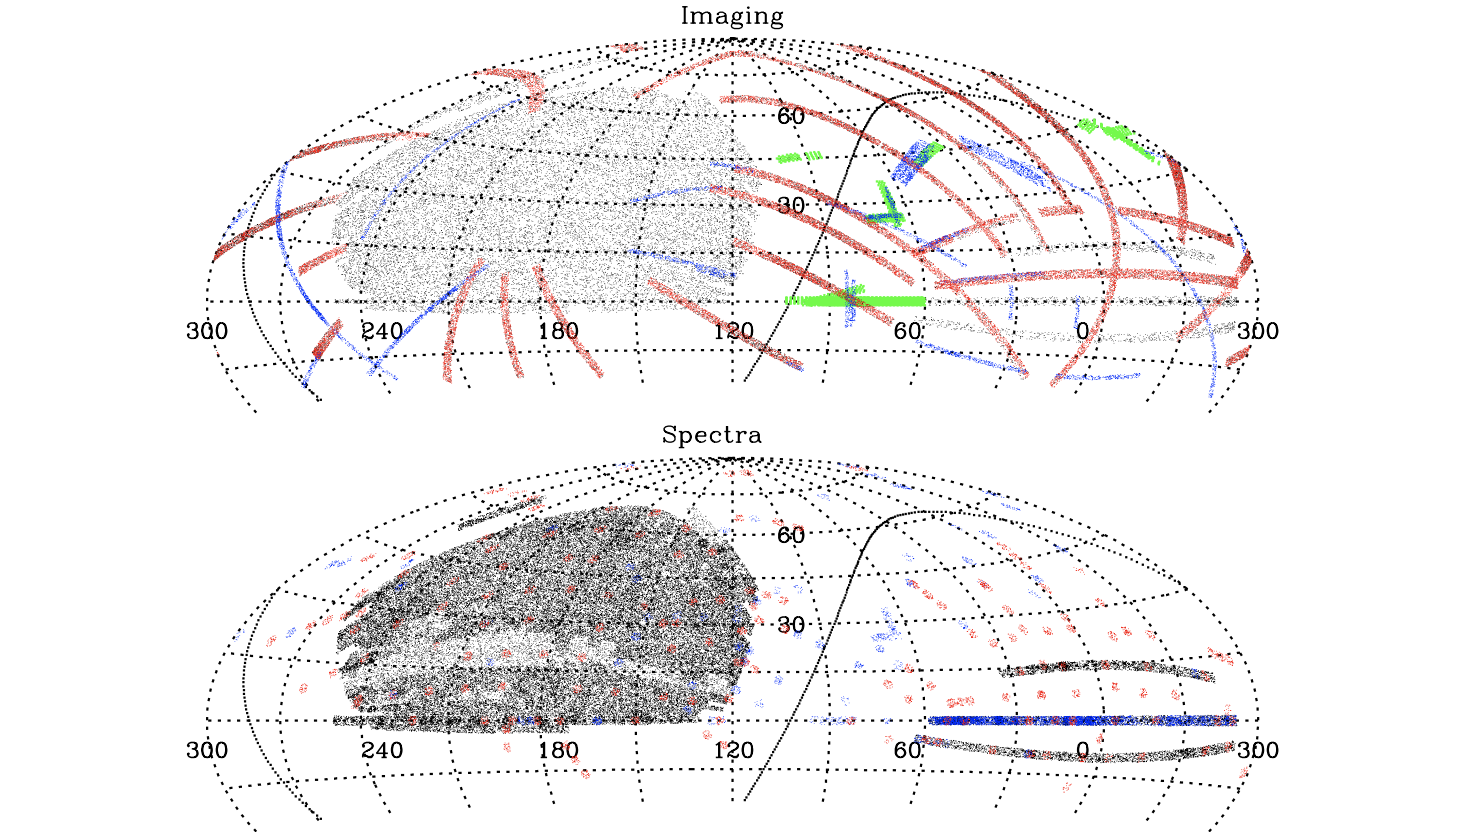
\includegraphics[width=1\textwidth]{SDSS_OFF}
  \caption{Distribution on the sky of the data included in DR7 (upper panel: imaging; lower panel: spectra), shown in an Aitoff equal-area projection in J2000 Equatorial Coordinates. The Galactic plane is the sinuous line that goes through each panel. \cite{2009ApJS..182..543A}}
  \label{3}
\end{figure}


\begin{comment}
 The first is a wide-field imager equipped with 24 tiles, each containing a 2048x2048 CCD. Imaging is performed along great circles at the sidereal rate, leading to exposure times of 54.1 seconds.

The astrometry is good to 45 milliarcseconds (mas) rms per coordinate at the bright end, while the photometric calibration is made in two modalities, respectively by tying to standard reference stars and by using the overlap between adjacent imaging runs in a process called ubercalibration.

Spectra are extracted and calibrated in terms of wavelength and flux. For galaxies near the main sample flux limit, the typical signal-to-noise ratio (S/N) is 10 per pixel. The broadband spectrophotometric calibration exhibits an accuracy of $4\%$ root mean square (rms) for point sources (Adelman-McCarthy et al. 2008), and the wavelength calibration is precise to $2 \, \text{km s}^{-1}$.

The SDSS data have been made public in a series of yearly data releases, This thesis works based its results from a galactic sample derived from "Data Release 7" by the Max Planck Institute for Astrophysics and Johns Hopkins University ( MPA-JHU )  teams, containing the derived properties of a total of 927'552 galaxy spectra.


\textbf{Physical Properties of interest :}
\begin{itemize}
		\item \textbf{Line Flux :}Flux from Gaussian fit to continuum subtracted data, corrected for foreground (galactic) reddening using techniques developed by O'Donnell \cite{1994ApJ...422..158O}
		\item \textbf{Error Line Flux :} Developed by analyzing the duplicate observations of galaxies, to compare the empirical spread in value determinations with the random errors.

\end{itemize}

\end{comment}


\subsection{C4 BCG Catalogue}
The identification of BCGs within our primary galaxy sample, previously described, relies on the BCG catalogue created by A. Von der Linden et al. \cite{2007MNRAS.379..867V, 2009yCat..73790867V}. This sample is derived from the further analysis of the C4 Galaxy Cluster Catalog,  developed by Miller et Al.  \cite{2005AJ....130..968M}.

The C4 catalog comprises 1106 galaxy clusters identified in the Third Data Release (DR3) of SDSS spanning redshifts from 0.02 to 0.16. 

In this context, the work by Von Der Linden et al.  \cite{2007MNRAS.379..867V} is noteworthy, as it builds upon the C4 catalog but introduces improved procedures for BCG identification and cluster velocity dispersion measurements, ultimately yielding a sample of 625 BCGs.

Despite primarily serving as a cluster catalogue, the original C4 also offered potential BCG candidates by identifying both a \textit{spectroscopic} candidate and a \textit{mean} candidate within each cluster. However, subsequent research conducted by Von Der Linden et al. revealed that approximately $30\%$ of identified clusters missed the true BCG due to fiber collisions in the SDSS spectrometry.
To address this issue and to construct a specific BCG sample, Von der Linden's team initially limited the sample by imposing $z\leq 0.1$ in order to ensure that clusters span a large angular extent in comparison to the minimum distance between SDSS spectrometry fibres of $\sim55$ arcsec. 
At this redshift, the magnitude limit in the red band of the spectroscopic sample is approximately $M_{r} \approx -20$, encompassing an initial sample of 833 clusters. The subsequent selection process involved a specific procedure including the estimation of the virial radius, the selection of the two brightest galaxies within the projection of the mean galaxy, and the application of criteria such as the concentration index and redshift/color compatibility for the final BCG identification.
Throughout the computation, several galaxies were lost due to two main structural reasons : initial misclassification of stars and associations with multiple clusters. This led to the rejection of more than 101 clusters, leading to the final sample of 625 elements.



\subsection{The Radio Catalogue}

I also exploit the radio catalog obtained from Best et al., containing 2712 radio sources selected as Radio loud and star-forming \cite{2005MNRAS.362....9B}. In order to study the fraction of the “BCG” and “non-BCG” samples it has been necessary to cross-match this catalog with that obtained from the match between SDSS and C4 in the previous section.
The Authors created this survey from the cross-match of a main spectroscopic galaxy sample and two radio surveys: the National Radio Astronomy Observatories (NRAO) Very Large Array (VLA) Sky Survey (NVSS) \cite{1998AJ....115.1693C} and the Faint Images of the Radio Sky at Twenty centimeters (FIRST) \cite{1995ApJ...450..559B}.


The NVSS was the first radio survey with an angular resolution of 45 arcsec. 
The FIRST catalogue offers angular resolution of 5 arcsec. Nonetheless, the high angular resolution of FIRST presents its own challenges, as it is insensitive to extended radio structures and resolves out the extended emission of radio sources. Consequently, the total radio luminosity of sources larger than a few arcseconds is systematically underestimated by FIRST. To address these limitations, a hybrid approach utilizing both NVSS and FIRST surveys has been developed to identify radio sources associated with galaxies in the SDSS spectroscopic sample. This approach capitalizes on the sensitivity of NVSS to large-scale radio structures and the high angular resolution of FIRST to reliably pinpoint the host galaxy.

The obtained radio source sample demonstrated a completeness of $95\%$ and a reliability of $98.9\%$, upgrading the achievable performance of each individual survey. The sample was subsequently classified into two groups: radio-loud active galactic nuclei (AGN) and galaxies where radio emission is predominantly driven by star formation. Classification was based on galaxies' positions in the plane of 4000 $\AA$ break strength versus radio luminosity per unit stellar mass, resulting in a dataset of 2,215 radio-loud AGN and 497 star-forming galaxies with radio luminosity exceeding 5 mJy at 1.4 GHz. \cite{2005MNRAS.362....9B, 10.1111/j.1365-2966.2005.09192.x}



\begin{comment}
This catalog is used to investigate the presence of radio counterpart of BCG and normal galaxies in the main SDSS catalogue, therefore, this is cross-matched with a main spectroscopic galaxy sample and two radio surveys: the National Radio Astronomy Observatories (NRAO) Very Large Array (VLA) Sky Survey (NVSS) \cite{1998AJ....115.1693C} and the Faint Images of the Radio Sky at Twenty centimeters (FIRST) survey \cite{1995ApJ...450..559B}.
\end{comment}


\begin{comment}
To investigate the radio emission characteristics of both BCGs and non-BCGs, this study conducted a crossmatch between the primary SDSS sample and a dataset comprising 2,712 radio-luminous galaxies from the work by \cite{2005MNRAS.362....9B}. This collection of radio-luminous objects resulted from a complex cross-matching process involving the main spectroscopic galaxy sample and two radio surveys: the National Radio Astronomy Observatories (NRAO) Very Large Array (VLA) Sky Survey (NVSS) \cite{1998AJ....115.1693C} and the Faint Images of the Radio Sky at Twenty centimeters (FIRST) survey. \cite{1995ApJ...450..559B}

The NVSS was the first radio survey with a sufficiently high angular resolution (45 arcsec) to allow automated cross-correlation with optical surveys. However, the FIRST catalogue offers superior angular resolution (approximately 5 arcsec), resulting in samples with much higher reliability. Nonetheless, the high angular resolution of FIRST presents its own challenges, as it is insensitive to extended radio structures and resolves out the extended emission of radio sources. Consequently, the total radio luminosity of sources larger than a few arcseconds is systematically underestimated by FIRST. To address these limitations, a hybrid approach utilizing both NVSS and FIRST surveys has been developed to identify radio sources associated with galaxies in the SDSS spectroscopic sample. This approach capitalizes on the sensitivity of NVSS to large-scale radio structures and the high angular resolution of FIRST to reliably pinpoint the host galaxy.

The obtained radio source sample demonstrated a completeness of $95\%$ and a reliability of $98.9\%$, upgrading the achievable performance of each individual survey. The sample was subsequently classified into two groups: radio-loud active galactic nuclei (AGN) and galaxies where radio emission is predominantly driven by star formation. Classification was based on a galaxy's position in the 4000-Å break strength versus radio luminosity per unit stellar mass plane, resulting in a dataset of 2,215 radio-loud AGN and 497 star-forming galaxies with radio luminosity exceeding 5 mJy at 1.4 GHz.
\end{comment}

\newpage
\section{Data Analysis}
The initial step of the analysis involved cross-matching the catalog of galaxy properties from the MPA-JHU emission line analysis for the SDSS DR7 with the C4 BCG sample, presented in the previous chapter, in order to identify the BCG candidates. In particular, using coordinates of the galaxies in both these samples, I selected galaxies in the SDSS catalog closest to the individual BCGs in the C4 catalog, within a distance of less than 2 arcseconds (i.e. the PSF of 1.4 arcsec). 
A distinct catalog was created for galaxies selected as “non-BCG”, which were exclusively chosen from within the cross-matched region of these surveys to minimize contamination from BCGs not included in the C4 catalog. 

At the end, through this process, i obtained two distinct samples, each containing comprehensive spectral properties for a total of 404 and 389454 galaxies identified as BCG and non-BCG, respectively. 
In \autoref{Cross:SDSS/C4} I report the distribution of galaxies from SDSS DR7 in grey and the BCGs identified from the crossmatch in red. The black dashed squares show the cross-matched area used to produce the BCG and non-BCG samples.

\begin{figure}[hbtp]
  \centering
  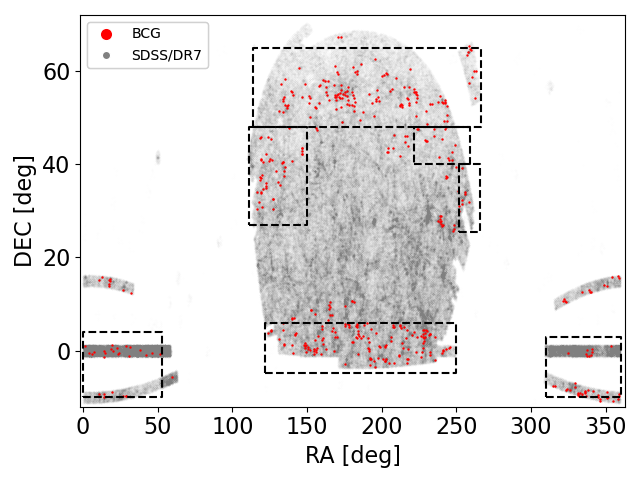
\includegraphics[width=0.8\textwidth]{BCGcmSDSS}
  \caption{Distribution of data on the sky in J2000 Equatorial Coordinates. The grey areas represent galaxies included in the main sample \cite{mpa-sdss-dr7}, while BCGs identified through crossmatching are highlighted in red. Dashed lines delineate the regions used for constructing the non-BCG sample. }
  \label{Cross:SDSS/C4}
\end{figure}

The final step in radio identification involves identifying galaxies exhibiting radio loud emission within both the BCG and non-BCG samples. This additional crossmatching process led to a refinement of the spatial regions, ensuring greater precision in excluding galaxies that may exhibit radio loudness but are not relevant to the radio survey under study. Based on the previously explained details regarding Radio survey's precision, galaxies displaying radio loudness were selected from the SDSS dataset within a distance of less than 5 arcsec. 

At the end, through this process, i obtained two distinct samples, each containing both spectral properties and radio loud detections, for a total of 409 and 365666 galaxies identified as BCG and non-BCG, respectively. In \autoref{8} i report the refined space regions needed for the determination of the radio loud fractions, together with a visual depiction of the BCGs and the Radio Emitters identified by cross-matching the catalogues. 

%% LA PARTE CHE AVEVO SCRITTO IO SULL'INTRODUZIONE AI DATI
\begin{comment}
As previously introduced, our primary galaxy sample for astrometry measurements is the MPA-JHU SDSS-derived catalogue.

The first operation required for the development of our study involved crossmatching the C4 BCG sample \cite{2009yCat..73790867V} to extract data files from the main sample, including both BCGs and non-BCGs.

This initial crossmatch was accomplished by selecting the nearest element within a radius of 2 arcsec in both RA and Dec corresponding to each of the BCGs in \cite{2009yCat..73790867V}. The result was a list of 484 corresponding selected elements.

At the end of this initial phase, the following data were collected for both samples:
\begin{itemize}
    \item \textbf{Astrometry data:} Celestial coordinates, Redshift, Error on redshift...
    \item \textbf{Spectroscopy measures:} Emission lines' fluxes and their relative errors
\end{itemize}
Even though further explanation is to follow, it is preferable to introduce the second crossmatch required for this work, this time with the 2712 galaxy samples of Celestial Objects found to be active in the radio field.

In this case, the research algorithm was designed to identify the nearest correspondence within a radius of 5 arcsec. The previously created files were appropriately updated by adding a specific flag, denoted as 1, to indicate whether, when found in the Radio Sample, it implies Radio Loud Emission.
\end{comment}
\subsection{Optical AGN Identification via BPT Diagram in BCG and non-BCG Samples}
In this section, we present an analysis aimed at detecting AGN activity within the galaxies in both the "BCG" and "non-BCG" samples.
To do it we use the Baldwin, Phillips $\&$ Terlevich (BPT) diagnostic diagram \cite{1981PASP...93....5B}.
This analysis is widely performed in literature to classify various types of galaxies based on the ratio of certain optical emission lines emitted form the gas within the host-galaxy, known as the inter-stellar medium (ISM). According to photoionization models, these line ratios are significantly influenced by the properties of the gas and its ionization level.
These specific ratios have been carefully chosen to prioritize similar wavelength fractions, minimizing dust attenuation. Specifically, this is developed based on the following ratios: \textbf{$\frac{[OIII]\lambda 5007}{H\beta}$}, \textbf{$\frac{[NII]\lambda 6583}{H\alpha}$}, \textbf{$\frac{[SII]\lambda\lambda 6716,6731}{H\alpha}$}, \textbf{$\frac{[OI]\lambda 6300}{H\alpha}$}.While the ideal classification incorporates all three primary BPT diagnostics, this study relies on a classification derived solely from the BPT diagrams for [NII] and [SII], based on the plot of $\frac{[OIII]\lambda 5007}{H\beta}$ versus  $\frac{[NII]\lambda 6583}{H\alpha}$ and $\frac{[NII]\lambda 6583}{H\alpha}$ versus $\frac{[SII]\lambda\lambda 6716,6731}{H\alpha}$, respectively.
According to different photoionization models it is possible to draw demarcation lines, that allow to classify the final objects into different categories : 

\begin{itemize}
    \item \textbf{BPT-[NII]:}

		\begin{itemize}
    		\item \textbf{Star-forming (SF):} where the ionization is primarily from massive stars.
    		\item \textbf{AGN (Active Galactic Nuclei):} Above both of the demarcation lines, delineating ionization by an active nucleus.
    		\item \textbf{Composite:} Galaxies exhibiting a mix of both star-forming and AGN characteristics, probably due to transition. Generally recognized to be in the area between both of the demarcation lines.
		\end{itemize}

		\item \textbf{BPT-[SII]:}
	\begin{itemize}
    		\item \textbf{Seyferts:} Above of both of the demarcation lines, characterized by high ionization levels.
    		\item \textbf{LINERs (Low-Ionization Nuclear Emission Regions):} Above the Main AGN line, and below LINER/Sy2.  Typically characterized by weak AGN-like ionization.
    		\item \textbf{Star-forming :} The primary source of ionization comes from the stars compounding the galaxy.
		\end{itemize}

\end{itemize}



The underlying concept of this method is rooted in an intrinsic property of the ionization spectrum of massive stars near the Lyman limit of Helium, found at $\lambda = 228\AA$. Massive stars exhibit a bright cut, while the non-thermal radiation of AGNs extends to higher energies. 

As a result, AGN host galaxies typically show greater ratios that surpass the demarcation lines predicted by photoionization models.

There were several photoionization models at the inception of this technique; nowadays, the preferred ones are Kauffmann et al. \cite{2003MNRAS.346.1055K} and Kewley et al. \cite{2001ApJ...556..121K}.

While the ideal classification incorporates all three primary BPT diagnostics, this study relies on a classification derived solely from the BPT diagrams for [NII] and [SII].

\begin{itemize}
    \item \textbf{BPT-[NII] Demarcation Functions:}
    \begin{itemize}
        \item Kauffmann+03 Line: \[ \text{log}(\frac{\text{[OIII]}}{\text{H}\beta}) = 0.61 / (\text{log}(\frac{\text{[NII]}}{\text{H}\alpha}) - 0.05) + 1.3 \]
        \item Kewley+01 Line: \[ \text{log}(\frac{\text{[OIII]}}{\text{H}\beta}) = 0.61 / (\text{log}(\frac{\text{[NII]}}{\text{H}\alpha}) - 0.47) + 1.19 \]
    \end{itemize}

    \item \textbf{BPT-[SII] Demarcation Functions:}
    \begin{itemize}
        \item Main AGN Line: \[ \text{log}(\frac{\text{[OIII]}}{\text{H}\beta}) = 0.72 / (\text{log}(\frac{\text{[SII]}}{\text{H}\alpha}) - 0.32) + 1.30 \]
        \item LINER/Sy2 Line: \[ \text{log}(\frac{\text{[OIII]}}{\text{H}\beta}) = 1.89 \text{log}(\frac{\text{[SII]}}{\text{H}\alpha}) + 0.76 \]
    \end{itemize}
\end{itemize}



Returning to the methodology employed in this thesis, an initial screening process was conducted to exclude objects with flux values that rendered logarithmic ratios incalculable, specifically eliminating instances with numerators or denominators equal to zero. Subsequently, scatterplots were generated and demarcation lines were applied to discern distinct galaxy populations.
Results images can be seen in :

\autoref{4} \autoref{5} \autoref{6} \autoref{7}

Given the inclusion of error values for each flux measurement, a robust bootstrap algorithm was implemented through 5000 iterations. This algorithm introduced variations to each point on the diagnostic diagram in two dimensions based on its probability distribution, with the mean value reflecting the error-free point and a standard deviation equivalent to the error associated with the point in both directions.

This rigorous approach facilitated an accurate determination of counts and fractions for all populations, providing a statistically refined measure of uncertainty.
\vspace{2cm}
\begin{figure}[hbtp]
  \centering
  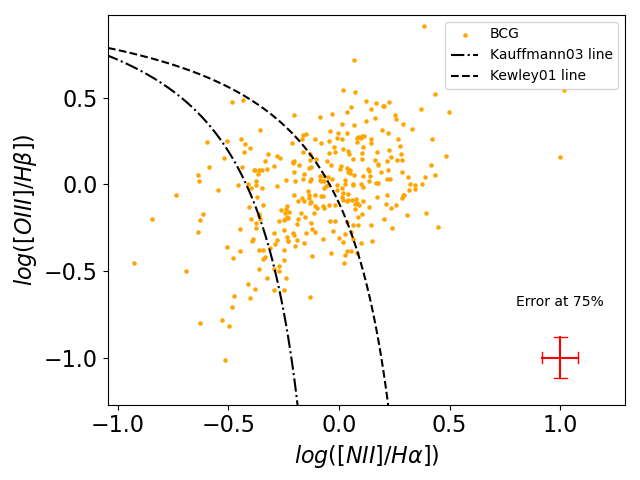
\includegraphics[width=0.65\textwidth]{BCG-NII-V22}
  \caption{BPT NII for the BCG sample }
  \label{4}
\end{figure}

\begin{figure}[hbtp]
  \centering
  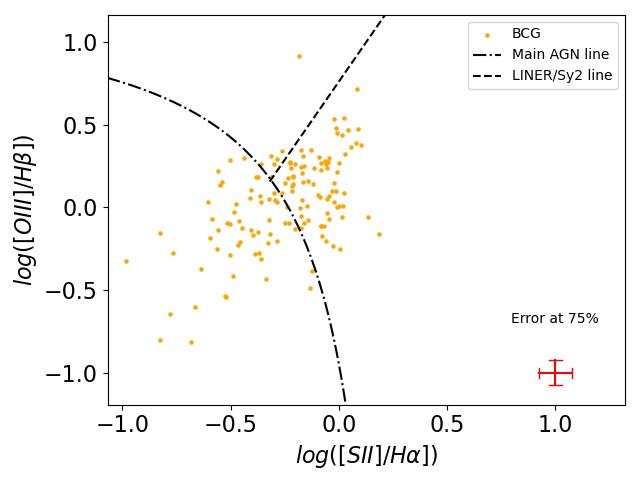
\includegraphics[width=0.65\textwidth]{BCG-SII1731-V22}
  \caption{BPT SII for the BCG sample }
  \label{5}
\end{figure}


\begin{figure}[hbtp]
  \centering
  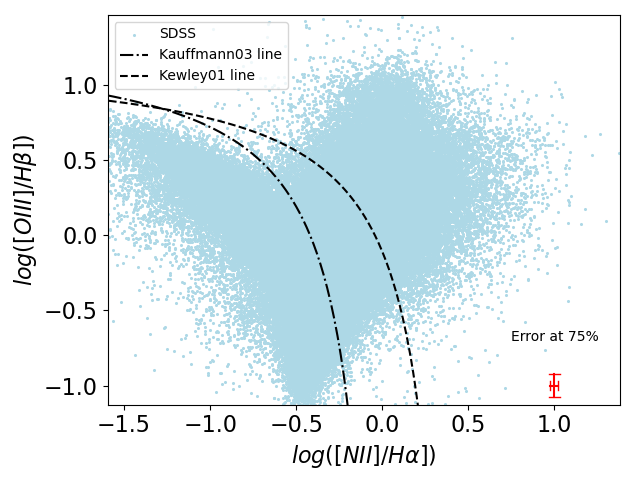
\includegraphics[width=0.7\textwidth]{SDSS-NII-V22}
  \caption{BPT NII for the SDSS noBCG sample }
  \label{6}
\end{figure}

\begin{figure}[hbtp]
  \centering
  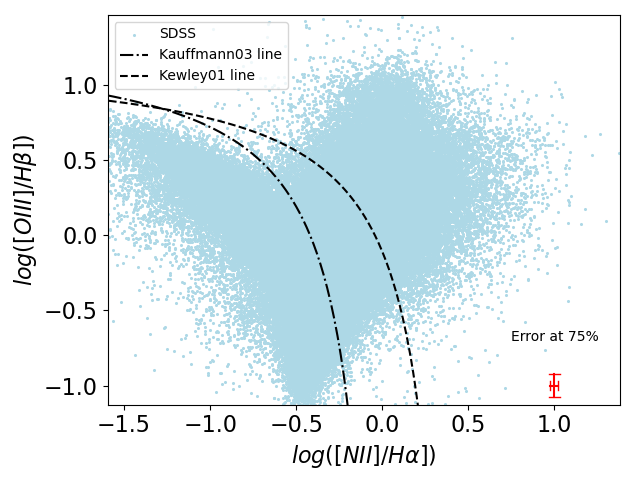
\includegraphics[width=0.7\textwidth]{SDSS-NII-V22}
  \caption{BPT SII for the SDSS noBCG sample }
  \label{7}
\end{figure}

\newpage
\subsection{Radio AGN activity in BCG and non-BCG galaxies}

Following the preceding analyses, let's now detail how the fractions of Radio Loud AGNs were calculated for the two derived samples.

The primary goal of this analysis segment is to determine a fraction of the form :
 $$\frac{N_{\text{radio}}}{N_{\text{total}}}$$

A crucial step in calculating a representative fraction of Radio Loud objects was to appropriately define the spatial regions for the fraction calculations. To accomplish this, we identified the regions mapped by the radio survey employed. Subsequently, the selection has been delineated where all three catalogs exhibited an overlap. It is essential to emphasize that the primary objective is to obtain representative fractions for both of our samples.

The selected spatial regions considered for calculating the fractions of Radio Loud objects can be found in \autoref{8}

\vspace{2cm}
\begin{figure}[hbtp]
  \centering
  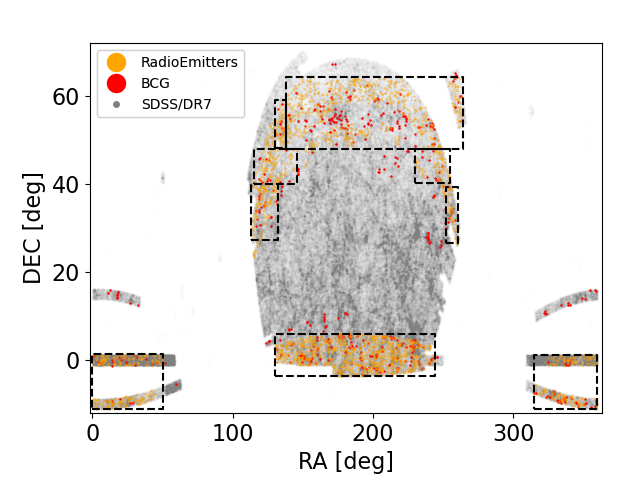
\includegraphics[width=0.9\textwidth]{Fourth}
  \caption{Distribution of data on the sky in J2000 Equatorial Coordinates. The grey areas depict galaxies included in the main sample \cite{mpa-sdss-dr7}, while BCGs identified through crossmatching are highlighted in red. Sources of radio emission found by Best et al. \cite{2005MNRAS.362....9B} are shown in orange. Dashed lines delineate the sky regions where the calculation of Radio Loud AGN fractions has been defined. }
  \label{8}
\end{figure}


 
